%\section{Introduction}

Laser frequency stabilisation is an essential tool for many atomic physics experiments~\cite{fox_1._2003,anderson_observation_1995,demarco_onset_1999,uetake_high_2008,ye_stable_2010,akamatsu_narrow_2012}.
There are a plethora of techniques available for laser frequency stabilisation each with numerous advantages and disadvantages.
Of particular interest here are stabilisation techniques that utilise high-bandwidth feedback to produce laser sources with narrow spectral linewidth which are important to applications such as atomic clocks~\cite{ludlow_sr_2008}, high-resolution spectroscopy~\cite{rafac_sub-dekahertz_2000}, and metrology~\cite{metcalf_laser_1999,ye_quantum_2008}.

Laser frequency stabilisation is an essential component of the \gls{caeis} as it is required for the \gls{mot} to function, for imaging of the atomic cloud and for the precise control involved in the ionisation process.
Relatively simple techniques such as saturated absorption spectroscopy~\cite{haroche_theory_1972,preston_doppler-free_1996,maguire_theoretical_2006} are adequate for the frequency linewidths required for the \gls{mot}.
More precise methods are useful when interacting with the Rydberg states of an atom as some of the Rydberg transitions have very narrow linewidths.

\Gls{pdh} locking with a high-finesse cavity~\cite{drever_laser_1983} is a proposed method for precise control over laser frequency.
\Gls{pdh} has been used to produce extremely good frequency stabilisation with sub-\unit[40]{mHz} linewidths achievable and is an essential part of the frequency stabilisation systems used at \gls{ligo}~\cite{ludlow_compact_2007,kessler_sub-40-mhz-linewidth_2012,abramovici_ligo:_1992,black_introduction_2001}.
The \gls{pdh} technique is unfortunately not relative to an absolute frequency reference, such as an atomic transition.
In order to capitalise on the narrow linewidth achievable with \gls{pdh} locking while ensuring absolute frequency stability, \gls{pdh} can be combined with saturation or polarisation spectroscopy to an absolute frequency reference such as an atomic transition, to prevent slower frequency drifts due to changes in the optical cavity resonance frequency as temperature and pressure changes in the lab.

The focus of this chapter is on \gls{ps} which was first described by Wieman and H\"anch in 1976 as, ``...a sensitive new method of Doppler-free spectroscopy, monitoring the nonlinear interaction of two monochromatic laser beams in an absorbing gas via changes in light polarisation."~\cite{wieman_doppler-free_1976,demtroder_laser_2003}.
It has been shown previously that \gls{ps} can be used to reduce the linewidth of a distributed feedback diode from \unit[2]{MHz} to \unit[20]{kHz}~\cite{torii_laser-phase_2012} and of an \gls{ecdl} to \unit[65]{kHz}~\cite{yoshikawa_frequency_2003}.
During the course of the research described here, \gls{ps} was demonstrated to be capable of linewidth reduction to sub-kilohertz linewidth if high-bandwidth feedback is used.
This work has been published as Reference~\cite{torrance_sub-kilohertz_2016}.

This chapter provides an overview of laser frequency stabilisation, a discussion of the physics of \gls{ps} followed by details on the implementation and measurement of high bandwidth frequency stabilisation using \gls{ps}.
Much of the work described in this chapter was conducted as part of an academic/industrial collaboration project with industry partner MOG Laboratories Pty. Ltd. ("MOGLabs").
The research outcomes were instrumental in improving the bandwidth of the electronics used within MOGLabs lasers which have since been used to achieve sub-hertz linewidths in a commercial system~\cite{menlo_systems_ors-dl_2016}.

\section{Laser Frequency Stabilisation}

Laser frequency stabilisation is used to reduce the frequency spread of a laser.
Laser frequency stabilisation can range from weak stabilisation keeping the centre frequency of a laser at a particular frequency to convoluted frequency narrowing techniques that attempt to reduce laser spectral linewidth to sub-hertz levels.
These techniques use a frequency reference such as an optical cavity or atomic transition and provide negative feedback to the laser, using a servo system, to keep the laser at the reference frequency.

A frequency discrimination method is used to generate an error signal and a servo system drives various feedback actuators to minimise that error.
A servo system is a system that uses error sensing negative feedback to control a device via an actuator.
A simple example of a servo is the cruise control in a car where the difference between the desired speed and the actual speed (the error signal) is used to modulate the throttle to get closer to the desired speed.
Laser stabilisation systems use servo systems to appropriately apply gain to the error signal and apply the result to the various feedback actuators available.

The efficacy of stabilisation techniques can be described by the width of the frequency distribution of the laser, called the linewidth.
Linewidth usually refers to either the \gls{fwhm} or \gls{rms} spectral width about the central frequency and is used to describe measurements made over various timescales.
Short duration measurements, usually less than a second, are used to describe the linewidth of lasers whereas long timescale measurement, hours or days in duration, are used to describe the drift of laser central frequency over time.

A number of traits are desirable in a laser frequency stabilisation scheme including:
\begin{itemize}
    \item \emph{Absolute frequency reference}: Frequency stabilisation techniques that rely on optical cavities are vulnerable to changes in the cavity resonant frequency, due to changes in cavity length with temperature or pressure for example, whereas other techniques such as \gls{sa} or \gls{ps} are relative to atomic energy levels and thus not subject to drift in the same way.
    \item \emph{High-bandwidth}: All else being equal, high-bandwidth techniques provide greater potential for linewidth reduction than low-bandwidth techniques.
    \item \emph{Modulation-free}: A number of stabilisation techniques require frequency- or phase-modulation which limits the bandwidth of the technique to half the modulation frequency due to the Nyquist limit; thus modulation-free, or high-frequency modulation techniques are often preferable. Modulation-free techniques are often more susceptible to low frequency noise than modulated techniques.
    \item \emph{Low drift}: Drift can occur with slow changes to the lock point of the stabilisation scheme, potentially due to ambient changes in lab temperature or pressure, or the electrical environment causing subsequent changes to laser beam power, polarisation or locking electronics voltage levels all of which can result in drift in the laser frequency. This can even occur with techniques that use an absolute frequency reference although non-absolute techniques tend to be more susceptible to drift.
    \item \emph{Stable}: Some techniques are more susceptible than others to unlocking, where perturbations such as ambient temperature or pressure changes, or percussive events (doors closing, dropped tools) cause large sudden changes in laser frequency which the servo system is unable to compensate for. Techniques with large capture ranges tend to have greater stability due to being able recover from larger frequency perturbations, see Section~\ref{section:capture_range} for an example.
\end{itemize}

There are a large number of available techniques and variations on techniques for stabilisation each with different advantages and drawbacks.
A few of these techniques are \gls{sa}~\cite{haroche_theory_1972, maguire_theoretical_2006, cuneo_optically_1994, preston_doppler-free_1996, saliba_linewidths_2009}, \gls{davll}~\cite{corwin_frequency-stabilized_1998, millett-sikking_davll_2007}, \gls{mts}~\cite{shirley_modulation_1982, mccarron_modulation_2008, xiang-hui_ultra-stable_2009,negnevitsky_wideband_2013}, Sagnac interferometry~\cite{robins_interferometric_2002, jundt_non-linear_2003}, \acrfull{ps}~\cite{wieman_doppler-free_1976, lancaster_polarisation_1999, yoshikawa_frequency_2003, harris_polarization_2006, pearman_polarization_2002, tiwari_laser_2006, do_polarization_2008, torii_laser-phase_2012}, \gls{pdh}~\cite{drever_laser_1983}, and H\"ansch Couillaud stabilisation~\cite{hansch_laser_1980}.

\subsection{Frequency Control and Feedback}

A number of methods can be used to control the output frequency of a laser and these can be used in concert to supply feedback from the frequency reference in order to stabilise the laser frequency and decrease the spectral linewidth.
The focus here will be on the feedback systems of diode lasers, particularly those of an \gls{ecdl}.

\subsubsection{Temperature}
The temperature of a laser diode affects the output frequency due to the temperature dependence of the optical path length, gain curves and the thermal expansion of the external cavity with an \gls{ecdl}~\cite{wieman_using_1991}.
The processes affect output frequency at different rates and all show an increase in wavelength with increasing temperature.

The temperature of laser diodes can be controlled through two methods. A \gls{tec} can be used to directly control the temperature of the device, and the injection current into the diode affects the temperature through resistive heating effects.
Good insulation and thermal inertia also contribute to the stability of diode temperature~\cite{saliba_cold_2011}.

Temperature is not typically used to directly manipulate the frequency of a laser due to the relatively slow response as changes in the control signal take seconds to propagate from the \gls{tec} to the diode and longer to fully thermalise.
Typically temperature is just stabilised to reduce the impact of ambient temperature changes on the performance of the diode laser.

\subsubsection{Injection Current}
Modulation of the injection current into the laser diode is one of most common ways of controlling the output wavelength of a diode laser.
The injection current into the diode affects the temperature of the diode, and the density of charge carriers which in turn affects the refractive index of the medium and thus the wavelength of the laser light produced.

Modulation of the injection current is the fastest feedback method available to diode lasers and is able to suppress noise up to \unit{MHz} ranges~\cite{ludlow_compact_2007,torrance_sub-kilohertz_2016}.
The design of the electronics involved in the modulation of the injection current can have a noticeable influence on the performance at high frequencies as noise becomes an issue.

The lasers used in the experiments described in this thesis all had two modes of current feedback, `slow' current feedback, with bandwidth from DC to approximately \unit[100]{kHz}, and `fast' current feedback, with bandwidth from about \unit[100]{kHz} to \unit[50]{MHz}.

The investigations of laser spectral behaviour, discussed later in this chapter, were instrumental in identifying potential improvements to the design of the electronics involved in the fast current channel of MOGLabs diode lasers.
The measurements presented were made with the final prototype of the enhanced laser headboard, now standard with lasers made by MOGLabs.

\subsubsection{Grating Angle and Position}
In external cavity diode lasers, for example the Littrow configuration \gls{ecdl} shown in Figure~\ref{figure:littrow}, the angle and position of the external grating can be used to control the output frequency.
The grating angle affects the wavelength of the light that is reflected back into the laser diode from the second-order reflection and thus the angle can be used to select output wavelength.
The grating position is used to control the length of the external cavity which also determines the laser wavelength and is commonly controlled using piezoelectric actuators~\cite{hawthorn_littrow_2001}.

\begin{figure}
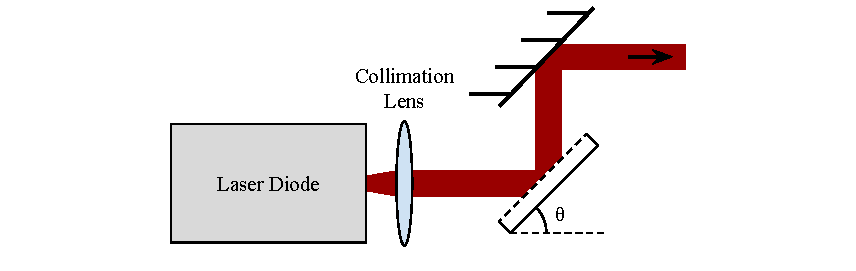
\includegraphics{part1/Figs/LittrowConfiguration.pdf}
\caption[Littrow configuration diode laser.]{Littrow configuration for diode lasers. The raw output of the diode is collimated and then incident on an optical grating. The angle of the grating, $\theta$, changes what frequency of light is coupled back into the diode from the first-order reflection and thus the frequency of output.}
\label{figure:littrow}
\end{figure}

Wavelength control via the grating angle is limited by the response rate of the piezo actuator which tend to respond in microseconds.
Thus the grating angle can be used to deal with relatively low frequency noise, up to approximately \unit[1]{kHz} or so, such as changes to ambient temperature, pressure, or some acoustic vibrations.

\subsection{Noise}
In this context noise refers to effects that change the frequency of a laser in undesirable ways.
Some sources of noise are thermal changes, ambient vibrations, atmospheric pressure, or the electrical power supply.

Thermal noise can be caused by a number of effects such as changes in weather or unreliable building climate control.
Thermal noise can directly affect the length of the laser cavity and the refractive index of air within the cavity but also affects the alignment of optics, the efficiency and polarisation of light transmitted through fibres, and atomic vapour cell opacity which can erroneously be interpreted by some frequency stabilisation systems as frequency changes and `corrected'.

Electrical noise can occur with changes to the wider electrical grid as well as when devices in the lab are turned on or off, fast switching high-voltage/-current supplies, such as those used to switch the \gls{mot} coils, can cause noticeable effects on other electrical equipment in close proximity.
Noise in the electronic environment can cause frequency instability particularly if a laser diode is not fully isolated from the electrical ground.
Noise on the power supply to the laser diode affects the power and frequency of the light emitted.
Laser intensity noise can also cause problems, for example laser frequency stabilisation is often conducted with spectroscopic techniques that will interpret intensity fluctuations as frequency fluctuations. Thus the feedback system will create frequency noise as it attempts to correct for the phantom frequency noise.

Mechanical noise can have numerous sources such as audible noise, percussive noise (dropped spanners, doors) or vibrational sources such as cooling fans on nearby equipment.
An \gls{ecdl} subjected to mechanical vibrations will experience frequency noise as the diode cavity length and refractive index varies.
Mechanical noise can also affect the alignment, and thus transmitted power, of light through optical fibres, optical isolators and apertures, which in turn can be falsely interpreted by the servo system as a change in frequency and `corrected'.

\section{Saturated Absorption Spectroscopy}
\glsreset{sa}
\Gls{sa} is a simple and common technique for laser frequency stabilisation which can be used with a number of atomic species and is a staple of atom optics laboratories~\cite{demtroder_laser_2003}.
\Gls{sa} is often used in applications where extremely narrow linewidths are not required due to the relative simplicity of the method such as \gls{mot} trapping and cooling, or atom cloud imaging.
A schematic of \gls{sa} is shown in Figure~\ref{figure:satabs}.

\begin{figure}
\center
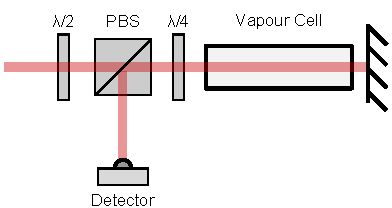
\includegraphics{part1/Figs/SatAbs.pdf}
\caption[Saturated absorption spectroscopy setup.]{An example of a saturated absorption spectroscopy setup. $\lambdaup$/2 and $\lambdaup$/4 refer to half- and quarter wave phase retarders respectively and are used to control the intensity of the light travelling through the vapour cell and hitting the detector using the \gls{pbs}.}
\label{figure:satabs}
\end{figure}

\Gls{sa} involves counter-propagating pump and probe beams from the laser source through a sample of atomic vapour with the intensity of the probe beam after the gas measured by a photodetector.
Without the pump beam the absorption of the probe as a function of laser frequency would show peaks at the atomic transitions.
The width of the absorption peaks is equal to the linewidth of each transition, broadened by the thermal distribution of the atoms due to thermal motion.
At room temperature the absorption spectrum for rubidium is a smooth curve 100s of MHz wide which obscures the hyperfine transitions.
Adding the pump beam results in less absorption at each transition due to the pump exciting atoms which are then inaccessible to the probe. With counter-propagating beams `cross-over' features appear halfway between each pair of transitions~\cite{demtroder_laser_2003}.
An example spectrum for rubidium-85 is shown in Figure~\ref{figure:satabsspectrum}.
In Figure~\ref{figure:satabs} the pump beam is recycled to act as the probe.

\begin{figure}
    \center
    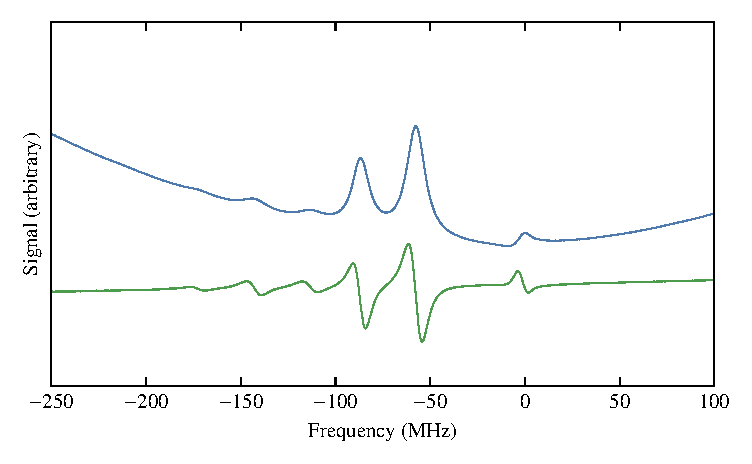
\includegraphics{part1/Figs/SatAbsSpectrum.pdf}
    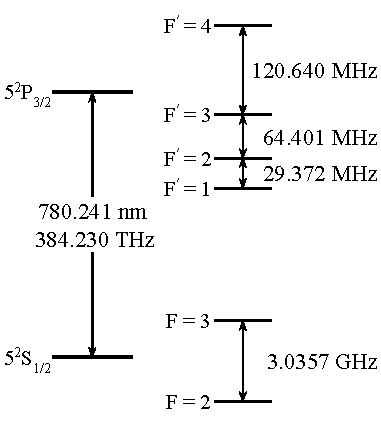
\includegraphics{part1/Figs/Rb85_D2_Energy_Levels.pdf}
    \caption[Saturated absorption spectroscopy absorption spectrum.]{An example of a saturated absorption spectroscopy absorption spectrum for the rubidium-85 D2 transition.
    The blue line shows the absorption spectrum and the green line shows the error signal for modulated \gls{sa}.
    From left to right the peaks in the absorption spectrum are the $F=3$ to $F'=2,2/3,3,2/4,3/4$, and $4$, where $x/y$ refers to a crossover transition.
    The figure on the right shows the energy levels of the rubidium-85 D2 transition~\cite{steck_rubidium_2008}.}
    \label{figure:satabsspectrum}
    % Code and data in Code/PolSpec Code/Laser/Spectra for Paper/Grapher.py
\end{figure}

Different variations of \gls{sa} can operate with or without frequency modulation, which can be modulation of the laser (at the laser diode or just the beam with an \gls{aom} or \gls{eom}) or modulation of the transition frequencies of the atoms in the vapour cell (via a solenoid magnet wrapped around the vapour cell).
Without modulation the system is more susceptible to drift and there is a frequency offset from the centre of the atomic transition.
If modulation is used then there is the added complexity of implementing the modulation and the feedback bandwidth is limited to half the modulation frequency.
Laser linewidth under \unit[150]{kHz} is attainable with modulated saturated absorption spectroscopy~\cite{saliba_linewidths_2009}.

\section{Pound Drever Hall}
\glsreset{pdh}
The \gls{pdh} technique is the gold-standard for laser frequency linewidth reduction and has been used to achieve extremely low linewidth of less than \unit[40]{mHz}~\cite{kessler_sub-40-mhz-linewidth_2012}.
\Gls{pdh} uses an optical cavity as a frequency reference and a modulated beam and some electronics to generate the error signal for feedback to the laser~\cite{drever_laser_1983,black_introduction_2001}.
\Gls{pdh} is a phase sensitive measurement that compares the laser frequency with the light stored in the optical cavity and thus is not bandwidth limited by the spontaneous emission lifetime.
A schematic of a standard \gls{pdh} setup is shown in Figure~\ref{figure:pdh_schematic}.

\begin{figure}
\centering
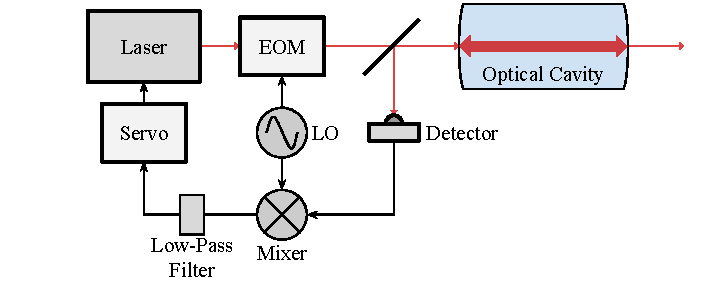
\includegraphics{part1/Figs/PDH.pdf}
\caption[Pound-Drever-Hall frequency stabilisation setup.]{A standard \gls{pdh} layout.
The laser beam passes through an \gls{eom} to create frequency sidebands and is then incident on the optical cavity.
The beam reflected from the cavity is detected with a photodetector and the signal passed through appropriate electronics to produce the error signal (see Section~\ref{section:pdh_error}).
The error signal is passed to the servo system to generate feedback to keep the laser frequency on the cavity resonance.}
\label{figure:pdh_schematic}
\end{figure}

\Gls{pdh} was used to provide a comparison to \gls{ps} and the optical cavity was used extensively as a diagnostic tool for examining laser frequency behaviour.

\subsection{Fabry-P\'erot Cavities}\label{section:cavity_theory}
A Fabry-P\'erot cavity is formed by two highly reflective mirrors facing each other such that light can form a standing wave between the two mirrors.
Laser light incident on a Fabry-P\'erot cavity will only couple into the cavity if the length of the cavity is equal to an integer number of wavelengths of the light.
So for an ideal laser to be resonant with an ideal cavity,
\begin{equation}
L = n \lambda,
\end{equation}
where $L$ is the length of the cavity, $\lambda$ is the wavelength of the laser and $n$ is some integer.
Realistic lasers and cavities have finite linewidths which when viewed as a transmission or reflection spectrum are shown as a convolution of the cavity and laser linewidth.

The frequency difference between one cavity transmission and the next is called the \gls{fsr}, $\Delta \nu_{FSR}$ and depends on the length of the cavity,
\begin{equation*}
\Delta \nu_{FSR} = \frac{c}{2L}
\end{equation*}
The quality of an optical cavity is described by the cavity finesse, $\mathscr{F}$, which effectively describes the number of traversals a beam makes before leaking out or being absorbed and it is determined by the intensity reflectivity of the mirrors, $R$,~\cite{hecht_optics_1987}
%\begin{align}
%\mathscr{F} &= \frac{2\pi}{-\log_e\left(R^2\right)} \notag\\
% &= \frac{\Delta \nu_{FSR}}{\delta},
%\end{align}
\begin{equation*}
\mathscr{F} = \pi\frac{\sqrt{R}}{1-R}.
\end{equation*}
%where $\delta$ is the \gls{fwhm} linewidth of the cavity.

The light transmitted through an optical cavity can be described by~\cite{pedrotti_introduction_2007}
\begin{equation}\label{equation:cavity_transmission}
T = \frac{1}{1+F\sin^2\frac{d}{2}},
\end{equation}
where $d=2\pi\frac{2L}{\lambda}$ and $F=\frac{4R}{\left(1-R\right)^2}$ is the coefficient of finesse.
The coefficient of finesse is related to the finesse by
\begin{equation}
\mathscr{F}=\frac{\pi}{2}\sqrt{F}.
\end{equation}
The phase difference between successive traversals of the cavity is represented by $d$.
We can define the difference between the laser wavelength and closest cavity resonance as $\Delta\lambda=L-n\lambda$, then Equation~\ref{equation:cavity_transmission} can be written as
\begin{align}\label{equation:cavity_transmission2}
T &= \frac{1}{1+F\sin^2\left(2\pi\frac{\Delta\lambda}{\lambda}\right)}. \notag \\
&\simeq \frac{1}{1+F\left(\frac{\omega L}{c}\right)^2},
\end{align}
where $\omega$ is the angular frequency of the laser.
$T$ takes the form of a Airy function and an example spectra is shown in Figure~\ref{figure:pdh_plots}.

We used a high-finesse cavity from Stable Laser Systems, isolated inside a temperature controlled vacuum chamber.
This cavity has a finesse of 20942, mirrors with a reflectivity of 0.99985, an \gls{fsr} of \unit[1.5]{GHz}, and a \gls{fwhm} linewidth of \unit[71.6]{kHz}.
This cavity had fixed mirrors unlike some others that have one of the mirrors attached to a piezoactuator to allow for modulation of the cavity resonance.

\subsubsection{PDH Error Signal}\label{section:pdh_error}

The magnitude of the optical electric field incident on a Fabry-P\'erot cavity, if the frequency is assumed to be approximately constant, can be written as
\begin{equation}
E_{I} = E_0 e^{i\omega t},
\end{equation}
where $\omega=2\pi f_l$ is the angular frequency of the laser.
The light reflected from the cavity consists of the promptly reflected beam and the leakage beam from light that has traversed the cavity one or more times before leaking out of the first mirror.
The promptly reflected beam undergoes a phase shift of $\pi$ relative to the incident beam.
The leakage beam has numerous phase components with one cavity round trip giving a phase shift of $-2L\omega/c$, two round trips giving $-4L\omega/c$, and so on.
Thus the reflected beam electric field will be
\begin{equation}\label{equation:cavity_reflected_field}
E_R = E_0 \left( r e^{i\left(\omega t + \pi\right)} + t r t e^{i\left(\omega t -2L\omega/c\right)} + t r^3 t e^{i\left(\omega t -4L\omega/c\right)} + ...\right),
\end{equation}
where $r$ is the mirror reflectivity and $t=\sqrt{1-r^2}$ is the transmissivity of the mirrors.
Equation~\ref{equation:cavity_reflected_field} can be simplified to give the reflection coefficient
\begin{equation}\label{equation:reflection_coefficient}
F_R(\omega) \equiv \frac{E_R}{E_I} = \frac{r\left(e^{i\omega / \Delta\nu_{FSR}} - 1 \right)}{1-r^2 e^{i\omega / \Delta\nu_{FSR}}}.
\end{equation}
Figure~\ref{figure:pdh_plots} shows that $F_R(\omega)$ is antisymmetric about the cavity resonance making it ideal for frequency stabilisation however more steps are required to generate a usable error signal.

To generate the error signal phase modulation is imposed on the laser beam, typically using an \gls{eom}.
The modulated incident laser beam with a modulation frequency of $\Omega$ and modulation strength $\beta$ has electric field
\begin{align}
E_I &= E_0 e^{i\left(\omega t + \beta \sin\Omega t \right)} \notag \\
&\approx E_0 \Bigg( J_0(\beta) + 2iJ_1(\beta)\sin\Omega t \Bigg)e^{i\omega t} \notag \\
&= E_0 \Bigg( J_0(\beta)e^{i\omega t} + J_1(\beta)e^{i(\omega + \Omega)t} - J_1(\beta)e^{i(\omega - \Omega)t} \Bigg),\label{equation:cavity_phase_mod}
\end{align}
valid for small $\beta$ where $J_0$ and $J_1$ are Bessel functions.
Equation~\ref{equation:cavity_phase_mod} shows that the phase modulated beam has three frequency components and the two $J_1$ components are referred to as the sidebands which are offset from the central frequency by the modulation frequency $\Omega$.

The reflected beam from the cavity due to the phase-modulated beam results in each frequency component being transformed by $F_R(\omega)$ to give
\begin{equation}
E_R = E_0 \Bigg(F_R(\omega)J_0(\beta)e^{i\omega t} + F_R(\omega+\Omega)J_1(\beta)e^{i(\omega+\Omega) t} - F_R(\omega-\Omega)J_1(\beta)e^{i(\omega-\Omega) t} \Bigg).
\end{equation}
The electric field is not directly measured, photodetectors measure the power, $P=|E|^2$, of the beam.
Thus,
\begin{align}
P_R \quad= \quad&P_c|F_R(\omega)|^2 \quad\qquad+\quad\qquad P_s \Bigg( F_R(\omega+\Omega) + F_R(\omega-\Omega)\bigg) &+\qquad&\notag\\
& 2\sqrt{P_cP_s} \, \operatorname{Re}\Bigg[ F_R(\omega)F_R^*(\omega+\Omega)-F_R^*(\omega)F_R(\omega-\Omega)\Bigg]\cdot\cos\Omega t &+\qquad& \notag\\
& 2\sqrt{P_cP_s} \, \operatorname{Im}\Bigg[ F_R(\omega)F_R^*(\omega+\Omega)-F_R^*(\omega)F_R(\omega-\Omega)\Bigg]\cdot\sin\Omega t &+ \qquad&O[2\Omega],\label{equation:pdh_detector}
\end{align}
where $P_{c,s}$ are the power of the carrier and sideband components respectively and the final term represents the higher-order components from the interactions between the sidebands.

The phase information is retrieved with the use of a ``mixer'' which is an electronic device that multiplies two signals together essentially multiplying the signal from the photodetector, $P_R \propto \sin\Omega t$, with the signal from the oscillator driving the \gls{eom}, $\sin\Omega t$.
The oscillating portions of the third and forth terms in Equation~\ref{equation:pdh_detector} when mixed become
\begin{align}
\cos\Omega t \sin\Omega t &= \frac{1}{2}\sin2\Omega \notag \\
\sin\Omega t \sin\Omega t &= \frac{1-\cos2\Omega t}{2},
\end{align}
thus resulting in a DC component and $2\Omega$ components.
A low-pass electronic filter is then used to extract the DC component which forms the \gls{pdh} error signal,
\begin{equation}\label{equation:pdh_error}
\epsilon = 2\sqrt{P_cP_s}\operatorname{Im}\Bigg[F_R(\omega)F_R^*(\omega+\Omega) - F_R^*(\omega)F_R(\omega-\Omega)\Bigg].
\end{equation}
An example \gls{pdh} error signal is shown in Figure~\ref{figure:pdh_plots}.
The steep antisymmetric slope about the resonance is ideal for frequency stabilisation and the large region, equal to twice the modulation frequency, about the resonance for which the signal is of the correct sign allows for a large capture range. 

\begin{figure}
\centering
%% Creator: Matplotlib, PGF backend
%%
%% To include the figure in your LaTeX document, write
%%   \input{<filename>.pgf}
%%
%% Make sure the required packages are loaded in your preamble
%%   \usepackage{pgf}
%%
%% Figures using additional raster images can only be included by \input if
%% they are in the same directory as the main LaTeX file. For loading figures
%% from other directories you can use the `import` package
%%   \usepackage{import}
%% and then include the figures with
%%   \import{<path to file>}{<filename>.pgf}
%%
%% Matplotlib used the following preamble
%%
\begingroup%
\makeatletter%
\begin{pgfpicture}%
\pgfpathrectangle{\pgfpointorigin}{\pgfqpoint{5.710000in}{1.903333in}}%
\pgfusepath{use as bounding box, clip}%
\begin{pgfscope}%
\pgfsetbuttcap%
\pgfsetmiterjoin%
\definecolor{currentfill}{rgb}{1.000000,1.000000,1.000000}%
\pgfsetfillcolor{currentfill}%
\pgfsetlinewidth{0.000000pt}%
\definecolor{currentstroke}{rgb}{1.000000,1.000000,1.000000}%
\pgfsetstrokecolor{currentstroke}%
\pgfsetdash{}{0pt}%
\pgfpathmoveto{\pgfqpoint{0.000000in}{0.000000in}}%
\pgfpathlineto{\pgfqpoint{5.710000in}{0.000000in}}%
\pgfpathlineto{\pgfqpoint{5.710000in}{1.903333in}}%
\pgfpathlineto{\pgfqpoint{0.000000in}{1.903333in}}%
\pgfpathclose%
\pgfusepath{fill}%
\end{pgfscope}%
\begin{pgfscope}%
\pgfsetbuttcap%
\pgfsetmiterjoin%
\definecolor{currentfill}{rgb}{1.000000,1.000000,1.000000}%
\pgfsetfillcolor{currentfill}%
\pgfsetlinewidth{0.000000pt}%
\definecolor{currentstroke}{rgb}{0.000000,0.000000,0.000000}%
\pgfsetstrokecolor{currentstroke}%
\pgfsetstrokeopacity{0.000000}%
\pgfsetdash{}{0pt}%
\pgfpathmoveto{\pgfqpoint{0.467472in}{0.521575in}}%
\pgfpathlineto{\pgfqpoint{1.794665in}{0.521575in}}%
\pgfpathlineto{\pgfqpoint{1.794665in}{1.691690in}}%
\pgfpathlineto{\pgfqpoint{0.467472in}{1.691690in}}%
\pgfpathclose%
\pgfusepath{fill}%
\end{pgfscope}%
\begin{pgfscope}%
\pgfpathrectangle{\pgfqpoint{0.467472in}{0.521575in}}{\pgfqpoint{1.327192in}{1.170115in}} %
\pgfusepath{clip}%
\pgfsetrectcap%
\pgfsetroundjoin%
\pgfsetlinewidth{1.003750pt}%
\definecolor{currentstroke}{rgb}{0.309804,0.478431,0.682353}%
\pgfsetstrokecolor{currentstroke}%
\pgfsetdash{}{0pt}%
\pgfpathmoveto{\pgfqpoint{0.467471in}{0.521681in}}%
\pgfpathlineto{\pgfqpoint{0.946189in}{0.522946in}}%
\pgfpathlineto{\pgfqpoint{1.015641in}{0.525086in}}%
\pgfpathlineto{\pgfqpoint{1.046191in}{0.528053in}}%
\pgfpathlineto{\pgfqpoint{1.063766in}{0.531844in}}%
\pgfpathlineto{\pgfqpoint{1.075398in}{0.536524in}}%
\pgfpathlineto{\pgfqpoint{1.083883in}{0.542280in}}%
\pgfpathlineto{\pgfqpoint{1.090583in}{0.549522in}}%
\pgfpathlineto{\pgfqpoint{1.096221in}{0.558984in}}%
\pgfpathlineto{\pgfqpoint{1.101183in}{0.571860in}}%
\pgfpathlineto{\pgfqpoint{1.105665in}{0.590041in}}%
\pgfpathlineto{\pgfqpoint{1.109769in}{0.616615in}}%
\pgfpathlineto{\pgfqpoint{1.113547in}{0.656773in}}%
\pgfpathlineto{\pgfqpoint{1.117038in}{0.719627in}}%
\pgfpathlineto{\pgfqpoint{1.120296in}{0.822112in}}%
\pgfpathlineto{\pgfqpoint{1.123426in}{0.997982in}}%
\pgfpathlineto{\pgfqpoint{1.126875in}{1.335073in}}%
\pgfpathlineto{\pgfqpoint{1.131000in}{1.691554in}}%
\pgfpathlineto{\pgfqpoint{1.131073in}{1.691689in}}%
\pgfpathlineto{\pgfqpoint{1.131144in}{1.691525in}}%
\pgfpathlineto{\pgfqpoint{1.131144in}{1.691525in}}%
\pgfpathlineto{\pgfqpoint{1.131561in}{1.684646in}}%
\pgfpathlineto{\pgfqpoint{1.132667in}{1.621579in}}%
\pgfpathlineto{\pgfqpoint{1.135831in}{1.268959in}}%
\pgfpathlineto{\pgfqpoint{1.140165in}{0.903565in}}%
\pgfpathlineto{\pgfqpoint{1.144055in}{0.746389in}}%
\pgfpathlineto{\pgfqpoint{1.148148in}{0.663010in}}%
\pgfpathlineto{\pgfqpoint{1.152549in}{0.615151in}}%
\pgfpathlineto{\pgfqpoint{1.157305in}{0.585995in}}%
\pgfpathlineto{\pgfqpoint{1.162469in}{0.567310in}}%
\pgfpathlineto{\pgfqpoint{1.168126in}{0.554778in}}%
\pgfpathlineto{\pgfqpoint{1.174463in}{0.545976in}}%
\pgfpathlineto{\pgfqpoint{1.181851in}{0.539493in}}%
\pgfpathlineto{\pgfqpoint{1.190974in}{0.534507in}}%
\pgfpathlineto{\pgfqpoint{1.203030in}{0.530567in}}%
\pgfpathlineto{\pgfqpoint{1.220214in}{0.527450in}}%
\pgfpathlineto{\pgfqpoint{1.247025in}{0.525054in}}%
\pgfpathlineto{\pgfqpoint{1.294440in}{0.523330in}}%
\pgfpathlineto{\pgfqpoint{1.397172in}{0.522237in}}%
\pgfpathlineto{\pgfqpoint{1.727073in}{0.521707in}}%
\pgfpathlineto{\pgfqpoint{1.794666in}{0.521681in}}%
\pgfpathlineto{\pgfqpoint{1.794666in}{0.521681in}}%
\pgfusepath{stroke}%
\end{pgfscope}%
\begin{pgfscope}%
\pgfsetrectcap%
\pgfsetmiterjoin%
\pgfsetlinewidth{1.003750pt}%
\definecolor{currentstroke}{rgb}{0.000000,0.000000,0.000000}%
\pgfsetstrokecolor{currentstroke}%
\pgfsetdash{}{0pt}%
\pgfpathmoveto{\pgfqpoint{0.467472in}{0.521575in}}%
\pgfpathlineto{\pgfqpoint{1.794665in}{0.521575in}}%
\pgfusepath{stroke}%
\end{pgfscope}%
\begin{pgfscope}%
\pgfsetrectcap%
\pgfsetmiterjoin%
\pgfsetlinewidth{1.003750pt}%
\definecolor{currentstroke}{rgb}{0.000000,0.000000,0.000000}%
\pgfsetstrokecolor{currentstroke}%
\pgfsetdash{}{0pt}%
\pgfpathmoveto{\pgfqpoint{0.467472in}{0.521575in}}%
\pgfpathlineto{\pgfqpoint{0.467472in}{1.691690in}}%
\pgfusepath{stroke}%
\end{pgfscope}%
\begin{pgfscope}%
\pgfsetrectcap%
\pgfsetmiterjoin%
\pgfsetlinewidth{1.003750pt}%
\definecolor{currentstroke}{rgb}{0.000000,0.000000,0.000000}%
\pgfsetstrokecolor{currentstroke}%
\pgfsetdash{}{0pt}%
\pgfpathmoveto{\pgfqpoint{0.467472in}{1.691690in}}%
\pgfpathlineto{\pgfqpoint{1.794665in}{1.691690in}}%
\pgfusepath{stroke}%
\end{pgfscope}%
\begin{pgfscope}%
\pgfsetrectcap%
\pgfsetmiterjoin%
\pgfsetlinewidth{1.003750pt}%
\definecolor{currentstroke}{rgb}{0.000000,0.000000,0.000000}%
\pgfsetstrokecolor{currentstroke}%
\pgfsetdash{}{0pt}%
\pgfpathmoveto{\pgfqpoint{1.794665in}{0.521575in}}%
\pgfpathlineto{\pgfqpoint{1.794665in}{1.691690in}}%
\pgfusepath{stroke}%
\end{pgfscope}%
\begin{pgfscope}%
\pgfsetbuttcap%
\pgfsetroundjoin%
\definecolor{currentfill}{rgb}{0.000000,0.000000,0.000000}%
\pgfsetfillcolor{currentfill}%
\pgfsetlinewidth{0.501875pt}%
\definecolor{currentstroke}{rgb}{0.000000,0.000000,0.000000}%
\pgfsetstrokecolor{currentstroke}%
\pgfsetdash{}{0pt}%
\pgfsys@defobject{currentmarker}{\pgfqpoint{0.000000in}{0.000000in}}{\pgfqpoint{0.000000in}{0.055556in}}{%
\pgfpathmoveto{\pgfqpoint{0.000000in}{0.000000in}}%
\pgfpathlineto{\pgfqpoint{0.000000in}{0.055556in}}%
\pgfusepath{stroke,fill}%
}%
\begin{pgfscope}%
\pgfsys@transformshift{0.777151in}{0.521575in}%
\pgfsys@useobject{currentmarker}{}%
\end{pgfscope}%
\end{pgfscope}%
\begin{pgfscope}%
\pgfsetbuttcap%
\pgfsetroundjoin%
\definecolor{currentfill}{rgb}{0.000000,0.000000,0.000000}%
\pgfsetfillcolor{currentfill}%
\pgfsetlinewidth{0.501875pt}%
\definecolor{currentstroke}{rgb}{0.000000,0.000000,0.000000}%
\pgfsetstrokecolor{currentstroke}%
\pgfsetdash{}{0pt}%
\pgfsys@defobject{currentmarker}{\pgfqpoint{0.000000in}{-0.055556in}}{\pgfqpoint{0.000000in}{0.000000in}}{%
\pgfpathmoveto{\pgfqpoint{0.000000in}{0.000000in}}%
\pgfpathlineto{\pgfqpoint{0.000000in}{-0.055556in}}%
\pgfusepath{stroke,fill}%
}%
\begin{pgfscope}%
\pgfsys@transformshift{0.777151in}{1.691690in}%
\pgfsys@useobject{currentmarker}{}%
\end{pgfscope}%
\end{pgfscope}%
\begin{pgfscope}%
\pgftext[x=0.777151in,y=0.466019in,,top]{\fontsize{10.000000}{12.000000}\selectfont \(\displaystyle -\Omega\)}%
\end{pgfscope}%
\begin{pgfscope}%
\pgfsetbuttcap%
\pgfsetroundjoin%
\definecolor{currentfill}{rgb}{0.000000,0.000000,0.000000}%
\pgfsetfillcolor{currentfill}%
\pgfsetlinewidth{0.501875pt}%
\definecolor{currentstroke}{rgb}{0.000000,0.000000,0.000000}%
\pgfsetstrokecolor{currentstroke}%
\pgfsetdash{}{0pt}%
\pgfsys@defobject{currentmarker}{\pgfqpoint{0.000000in}{0.000000in}}{\pgfqpoint{0.000000in}{0.055556in}}{%
\pgfpathmoveto{\pgfqpoint{0.000000in}{0.000000in}}%
\pgfpathlineto{\pgfqpoint{0.000000in}{0.055556in}}%
\pgfusepath{stroke,fill}%
}%
\begin{pgfscope}%
\pgfsys@transformshift{1.131068in}{0.521575in}%
\pgfsys@useobject{currentmarker}{}%
\end{pgfscope}%
\end{pgfscope}%
\begin{pgfscope}%
\pgfsetbuttcap%
\pgfsetroundjoin%
\definecolor{currentfill}{rgb}{0.000000,0.000000,0.000000}%
\pgfsetfillcolor{currentfill}%
\pgfsetlinewidth{0.501875pt}%
\definecolor{currentstroke}{rgb}{0.000000,0.000000,0.000000}%
\pgfsetstrokecolor{currentstroke}%
\pgfsetdash{}{0pt}%
\pgfsys@defobject{currentmarker}{\pgfqpoint{0.000000in}{-0.055556in}}{\pgfqpoint{0.000000in}{0.000000in}}{%
\pgfpathmoveto{\pgfqpoint{0.000000in}{0.000000in}}%
\pgfpathlineto{\pgfqpoint{0.000000in}{-0.055556in}}%
\pgfusepath{stroke,fill}%
}%
\begin{pgfscope}%
\pgfsys@transformshift{1.131068in}{1.691690in}%
\pgfsys@useobject{currentmarker}{}%
\end{pgfscope}%
\end{pgfscope}%
\begin{pgfscope}%
\pgftext[x=1.131068in,y=0.466019in,,top]{\fontsize{10.000000}{12.000000}\selectfont 0}%
\end{pgfscope}%
\begin{pgfscope}%
\pgfsetbuttcap%
\pgfsetroundjoin%
\definecolor{currentfill}{rgb}{0.000000,0.000000,0.000000}%
\pgfsetfillcolor{currentfill}%
\pgfsetlinewidth{0.501875pt}%
\definecolor{currentstroke}{rgb}{0.000000,0.000000,0.000000}%
\pgfsetstrokecolor{currentstroke}%
\pgfsetdash{}{0pt}%
\pgfsys@defobject{currentmarker}{\pgfqpoint{0.000000in}{0.000000in}}{\pgfqpoint{0.000000in}{0.055556in}}{%
\pgfpathmoveto{\pgfqpoint{0.000000in}{0.000000in}}%
\pgfpathlineto{\pgfqpoint{0.000000in}{0.055556in}}%
\pgfusepath{stroke,fill}%
}%
\begin{pgfscope}%
\pgfsys@transformshift{1.484986in}{0.521575in}%
\pgfsys@useobject{currentmarker}{}%
\end{pgfscope}%
\end{pgfscope}%
\begin{pgfscope}%
\pgfsetbuttcap%
\pgfsetroundjoin%
\definecolor{currentfill}{rgb}{0.000000,0.000000,0.000000}%
\pgfsetfillcolor{currentfill}%
\pgfsetlinewidth{0.501875pt}%
\definecolor{currentstroke}{rgb}{0.000000,0.000000,0.000000}%
\pgfsetstrokecolor{currentstroke}%
\pgfsetdash{}{0pt}%
\pgfsys@defobject{currentmarker}{\pgfqpoint{0.000000in}{-0.055556in}}{\pgfqpoint{0.000000in}{0.000000in}}{%
\pgfpathmoveto{\pgfqpoint{0.000000in}{0.000000in}}%
\pgfpathlineto{\pgfqpoint{0.000000in}{-0.055556in}}%
\pgfusepath{stroke,fill}%
}%
\begin{pgfscope}%
\pgfsys@transformshift{1.484986in}{1.691690in}%
\pgfsys@useobject{currentmarker}{}%
\end{pgfscope}%
\end{pgfscope}%
\begin{pgfscope}%
\pgftext[x=1.484986in,y=0.466019in,,top]{\fontsize{10.000000}{12.000000}\selectfont \(\displaystyle \Omega\)}%
\end{pgfscope}%
\begin{pgfscope}%
\pgfsetbuttcap%
\pgfsetroundjoin%
\definecolor{currentfill}{rgb}{0.000000,0.000000,0.000000}%
\pgfsetfillcolor{currentfill}%
\pgfsetlinewidth{0.501875pt}%
\definecolor{currentstroke}{rgb}{0.000000,0.000000,0.000000}%
\pgfsetstrokecolor{currentstroke}%
\pgfsetdash{}{0pt}%
\pgfsys@defobject{currentmarker}{\pgfqpoint{0.000000in}{0.000000in}}{\pgfqpoint{0.055556in}{0.000000in}}{%
\pgfpathmoveto{\pgfqpoint{0.000000in}{0.000000in}}%
\pgfpathlineto{\pgfqpoint{0.055556in}{0.000000in}}%
\pgfusepath{stroke,fill}%
}%
\begin{pgfscope}%
\pgfsys@transformshift{0.467472in}{0.521575in}%
\pgfsys@useobject{currentmarker}{}%
\end{pgfscope}%
\end{pgfscope}%
\begin{pgfscope}%
\pgfsetbuttcap%
\pgfsetroundjoin%
\definecolor{currentfill}{rgb}{0.000000,0.000000,0.000000}%
\pgfsetfillcolor{currentfill}%
\pgfsetlinewidth{0.501875pt}%
\definecolor{currentstroke}{rgb}{0.000000,0.000000,0.000000}%
\pgfsetstrokecolor{currentstroke}%
\pgfsetdash{}{0pt}%
\pgfsys@defobject{currentmarker}{\pgfqpoint{-0.055556in}{0.000000in}}{\pgfqpoint{0.000000in}{0.000000in}}{%
\pgfpathmoveto{\pgfqpoint{0.000000in}{0.000000in}}%
\pgfpathlineto{\pgfqpoint{-0.055556in}{0.000000in}}%
\pgfusepath{stroke,fill}%
}%
\begin{pgfscope}%
\pgfsys@transformshift{1.794665in}{0.521575in}%
\pgfsys@useobject{currentmarker}{}%
\end{pgfscope}%
\end{pgfscope}%
\begin{pgfscope}%
\pgftext[x=0.411917in,y=0.521575in,right,]{\fontsize{10.000000}{12.000000}\selectfont \(\displaystyle 0\)}%
\end{pgfscope}%
\begin{pgfscope}%
\pgfsetbuttcap%
\pgfsetroundjoin%
\definecolor{currentfill}{rgb}{0.000000,0.000000,0.000000}%
\pgfsetfillcolor{currentfill}%
\pgfsetlinewidth{0.501875pt}%
\definecolor{currentstroke}{rgb}{0.000000,0.000000,0.000000}%
\pgfsetstrokecolor{currentstroke}%
\pgfsetdash{}{0pt}%
\pgfsys@defobject{currentmarker}{\pgfqpoint{0.000000in}{0.000000in}}{\pgfqpoint{0.055556in}{0.000000in}}{%
\pgfpathmoveto{\pgfqpoint{0.000000in}{0.000000in}}%
\pgfpathlineto{\pgfqpoint{0.055556in}{0.000000in}}%
\pgfusepath{stroke,fill}%
}%
\begin{pgfscope}%
\pgfsys@transformshift{0.467472in}{1.691690in}%
\pgfsys@useobject{currentmarker}{}%
\end{pgfscope}%
\end{pgfscope}%
\begin{pgfscope}%
\pgfsetbuttcap%
\pgfsetroundjoin%
\definecolor{currentfill}{rgb}{0.000000,0.000000,0.000000}%
\pgfsetfillcolor{currentfill}%
\pgfsetlinewidth{0.501875pt}%
\definecolor{currentstroke}{rgb}{0.000000,0.000000,0.000000}%
\pgfsetstrokecolor{currentstroke}%
\pgfsetdash{}{0pt}%
\pgfsys@defobject{currentmarker}{\pgfqpoint{-0.055556in}{0.000000in}}{\pgfqpoint{0.000000in}{0.000000in}}{%
\pgfpathmoveto{\pgfqpoint{0.000000in}{0.000000in}}%
\pgfpathlineto{\pgfqpoint{-0.055556in}{0.000000in}}%
\pgfusepath{stroke,fill}%
}%
\begin{pgfscope}%
\pgfsys@transformshift{1.794665in}{1.691690in}%
\pgfsys@useobject{currentmarker}{}%
\end{pgfscope}%
\end{pgfscope}%
\begin{pgfscope}%
\pgftext[x=0.411917in,y=1.691690in,right,]{\fontsize{10.000000}{12.000000}\selectfont \(\displaystyle 1\)}%
\end{pgfscope}%
\begin{pgfscope}%
\pgftext[x=0.273028in,y=1.106632in,,bottom,rotate=90.000000]{\fontsize{10.000000}{12.000000}\selectfont T}%
\end{pgfscope}%
\begin{pgfscope}%
\pgfsetbuttcap%
\pgfsetmiterjoin%
\definecolor{currentfill}{rgb}{1.000000,1.000000,1.000000}%
\pgfsetfillcolor{currentfill}%
\pgfsetlinewidth{0.000000pt}%
\definecolor{currentstroke}{rgb}{0.000000,0.000000,0.000000}%
\pgfsetstrokecolor{currentstroke}%
\pgfsetstrokeopacity{0.000000}%
\pgfsetdash{}{0pt}%
\pgfpathmoveto{\pgfqpoint{2.350140in}{0.521575in}}%
\pgfpathlineto{\pgfqpoint{3.677332in}{0.521575in}}%
\pgfpathlineto{\pgfqpoint{3.677332in}{1.691690in}}%
\pgfpathlineto{\pgfqpoint{2.350140in}{1.691690in}}%
\pgfpathclose%
\pgfusepath{fill}%
\end{pgfscope}%
\begin{pgfscope}%
\pgfpathrectangle{\pgfqpoint{2.350140in}{0.521575in}}{\pgfqpoint{1.327192in}{1.170115in}} %
\pgfusepath{clip}%
\pgfsetrectcap%
\pgfsetroundjoin%
\pgfsetlinewidth{1.003750pt}%
\definecolor{currentstroke}{rgb}{0.309804,0.478431,0.682353}%
\pgfsetstrokecolor{currentstroke}%
\pgfsetdash{}{0pt}%
\pgfpathmoveto{\pgfqpoint{2.350138in}{1.095470in}}%
\pgfpathlineto{\pgfqpoint{2.529255in}{1.091347in}}%
\pgfpathlineto{\pgfqpoint{2.643691in}{1.086630in}}%
\pgfpathlineto{\pgfqpoint{2.721528in}{1.081320in}}%
\pgfpathlineto{\pgfqpoint{2.777042in}{1.075414in}}%
\pgfpathlineto{\pgfqpoint{2.818153in}{1.068902in}}%
\pgfpathlineto{\pgfqpoint{2.849561in}{1.061763in}}%
\pgfpathlineto{\pgfqpoint{2.874219in}{1.053952in}}%
\pgfpathlineto{\pgfqpoint{2.894063in}{1.045397in}}%
\pgfpathlineto{\pgfqpoint{2.910416in}{1.035972in}}%
\pgfpathlineto{\pgfqpoint{2.924206in}{1.025487in}}%
\pgfpathlineto{\pgfqpoint{2.936102in}{1.013656in}}%
\pgfpathlineto{\pgfqpoint{2.946585in}{1.000071in}}%
\pgfpathlineto{\pgfqpoint{2.956008in}{0.984163in}}%
\pgfpathlineto{\pgfqpoint{2.964634in}{0.965130in}}%
\pgfpathlineto{\pgfqpoint{2.972683in}{0.941817in}}%
\pgfpathlineto{\pgfqpoint{2.980412in}{0.912331in}}%
\pgfpathlineto{\pgfqpoint{2.988474in}{0.872220in}}%
\pgfpathlineto{\pgfqpoint{2.999849in}{0.815338in}}%
\pgfpathlineto{\pgfqpoint{3.001346in}{0.814174in}}%
\pgfpathlineto{\pgfqpoint{3.001601in}{0.814371in}}%
\pgfpathlineto{\pgfqpoint{3.002790in}{0.817192in}}%
\pgfpathlineto{\pgfqpoint{3.004507in}{0.828170in}}%
\pgfpathlineto{\pgfqpoint{3.006752in}{0.859253in}}%
\pgfpathlineto{\pgfqpoint{3.009609in}{0.934277in}}%
\pgfpathlineto{\pgfqpoint{3.014093in}{1.123090in}}%
\pgfpathlineto{\pgfqpoint{3.019782in}{1.334075in}}%
\pgfpathlineto{\pgfqpoint{3.023102in}{1.386320in}}%
\pgfpathlineto{\pgfqpoint{3.025620in}{1.398568in}}%
\pgfpathlineto{\pgfqpoint{3.026768in}{1.399042in}}%
\pgfpathlineto{\pgfqpoint{3.027071in}{1.398774in}}%
\pgfpathlineto{\pgfqpoint{3.028641in}{1.395330in}}%
\pgfpathlineto{\pgfqpoint{3.031721in}{1.382056in}}%
\pgfpathlineto{\pgfqpoint{3.053316in}{1.276465in}}%
\pgfpathlineto{\pgfqpoint{3.061873in}{1.250605in}}%
\pgfpathlineto{\pgfqpoint{3.070907in}{1.230184in}}%
\pgfpathlineto{\pgfqpoint{3.080645in}{1.213552in}}%
\pgfpathlineto{\pgfqpoint{3.091319in}{1.199667in}}%
\pgfpathlineto{\pgfqpoint{3.103229in}{1.187810in}}%
\pgfpathlineto{\pgfqpoint{3.116771in}{1.177481in}}%
\pgfpathlineto{\pgfqpoint{3.132489in}{1.168331in}}%
\pgfpathlineto{\pgfqpoint{3.151114in}{1.160118in}}%
\pgfpathlineto{\pgfqpoint{3.173644in}{1.152684in}}%
\pgfpathlineto{\pgfqpoint{3.201471in}{1.145925in}}%
\pgfpathlineto{\pgfqpoint{3.236582in}{1.139778in}}%
\pgfpathlineto{\pgfqpoint{3.281899in}{1.134204in}}%
\pgfpathlineto{\pgfqpoint{3.341894in}{1.129180in}}%
\pgfpathlineto{\pgfqpoint{3.423666in}{1.124692in}}%
\pgfpathlineto{\pgfqpoint{3.539056in}{1.120730in}}%
\pgfpathlineto{\pgfqpoint{3.677334in}{1.117795in}}%
\pgfpathlineto{\pgfqpoint{3.677334in}{1.117795in}}%
\pgfusepath{stroke}%
\end{pgfscope}%
\begin{pgfscope}%
\pgfsetrectcap%
\pgfsetmiterjoin%
\pgfsetlinewidth{1.003750pt}%
\definecolor{currentstroke}{rgb}{0.000000,0.000000,0.000000}%
\pgfsetstrokecolor{currentstroke}%
\pgfsetdash{}{0pt}%
\pgfpathmoveto{\pgfqpoint{2.350140in}{0.521575in}}%
\pgfpathlineto{\pgfqpoint{3.677332in}{0.521575in}}%
\pgfusepath{stroke}%
\end{pgfscope}%
\begin{pgfscope}%
\pgfsetrectcap%
\pgfsetmiterjoin%
\pgfsetlinewidth{1.003750pt}%
\definecolor{currentstroke}{rgb}{0.000000,0.000000,0.000000}%
\pgfsetstrokecolor{currentstroke}%
\pgfsetdash{}{0pt}%
\pgfpathmoveto{\pgfqpoint{2.350140in}{0.521575in}}%
\pgfpathlineto{\pgfqpoint{2.350140in}{1.691690in}}%
\pgfusepath{stroke}%
\end{pgfscope}%
\begin{pgfscope}%
\pgfsetrectcap%
\pgfsetmiterjoin%
\pgfsetlinewidth{1.003750pt}%
\definecolor{currentstroke}{rgb}{0.000000,0.000000,0.000000}%
\pgfsetstrokecolor{currentstroke}%
\pgfsetdash{}{0pt}%
\pgfpathmoveto{\pgfqpoint{2.350140in}{1.691690in}}%
\pgfpathlineto{\pgfqpoint{3.677332in}{1.691690in}}%
\pgfusepath{stroke}%
\end{pgfscope}%
\begin{pgfscope}%
\pgfsetrectcap%
\pgfsetmiterjoin%
\pgfsetlinewidth{1.003750pt}%
\definecolor{currentstroke}{rgb}{0.000000,0.000000,0.000000}%
\pgfsetstrokecolor{currentstroke}%
\pgfsetdash{}{0pt}%
\pgfpathmoveto{\pgfqpoint{3.677332in}{0.521575in}}%
\pgfpathlineto{\pgfqpoint{3.677332in}{1.691690in}}%
\pgfusepath{stroke}%
\end{pgfscope}%
\begin{pgfscope}%
\pgfsetbuttcap%
\pgfsetroundjoin%
\definecolor{currentfill}{rgb}{0.000000,0.000000,0.000000}%
\pgfsetfillcolor{currentfill}%
\pgfsetlinewidth{0.501875pt}%
\definecolor{currentstroke}{rgb}{0.000000,0.000000,0.000000}%
\pgfsetstrokecolor{currentstroke}%
\pgfsetdash{}{0pt}%
\pgfsys@defobject{currentmarker}{\pgfqpoint{0.000000in}{0.000000in}}{\pgfqpoint{0.000000in}{0.055556in}}{%
\pgfpathmoveto{\pgfqpoint{0.000000in}{0.000000in}}%
\pgfpathlineto{\pgfqpoint{0.000000in}{0.055556in}}%
\pgfusepath{stroke,fill}%
}%
\begin{pgfscope}%
\pgfsys@transformshift{2.659818in}{0.521575in}%
\pgfsys@useobject{currentmarker}{}%
\end{pgfscope}%
\end{pgfscope}%
\begin{pgfscope}%
\pgfsetbuttcap%
\pgfsetroundjoin%
\definecolor{currentfill}{rgb}{0.000000,0.000000,0.000000}%
\pgfsetfillcolor{currentfill}%
\pgfsetlinewidth{0.501875pt}%
\definecolor{currentstroke}{rgb}{0.000000,0.000000,0.000000}%
\pgfsetstrokecolor{currentstroke}%
\pgfsetdash{}{0pt}%
\pgfsys@defobject{currentmarker}{\pgfqpoint{0.000000in}{-0.055556in}}{\pgfqpoint{0.000000in}{0.000000in}}{%
\pgfpathmoveto{\pgfqpoint{0.000000in}{0.000000in}}%
\pgfpathlineto{\pgfqpoint{0.000000in}{-0.055556in}}%
\pgfusepath{stroke,fill}%
}%
\begin{pgfscope}%
\pgfsys@transformshift{2.659818in}{1.691690in}%
\pgfsys@useobject{currentmarker}{}%
\end{pgfscope}%
\end{pgfscope}%
\begin{pgfscope}%
\pgftext[x=2.659818in,y=0.466019in,,top]{\fontsize{10.000000}{12.000000}\selectfont \(\displaystyle -\Omega\)}%
\end{pgfscope}%
\begin{pgfscope}%
\pgfsetbuttcap%
\pgfsetroundjoin%
\definecolor{currentfill}{rgb}{0.000000,0.000000,0.000000}%
\pgfsetfillcolor{currentfill}%
\pgfsetlinewidth{0.501875pt}%
\definecolor{currentstroke}{rgb}{0.000000,0.000000,0.000000}%
\pgfsetstrokecolor{currentstroke}%
\pgfsetdash{}{0pt}%
\pgfsys@defobject{currentmarker}{\pgfqpoint{0.000000in}{0.000000in}}{\pgfqpoint{0.000000in}{0.055556in}}{%
\pgfpathmoveto{\pgfqpoint{0.000000in}{0.000000in}}%
\pgfpathlineto{\pgfqpoint{0.000000in}{0.055556in}}%
\pgfusepath{stroke,fill}%
}%
\begin{pgfscope}%
\pgfsys@transformshift{3.013736in}{0.521575in}%
\pgfsys@useobject{currentmarker}{}%
\end{pgfscope}%
\end{pgfscope}%
\begin{pgfscope}%
\pgfsetbuttcap%
\pgfsetroundjoin%
\definecolor{currentfill}{rgb}{0.000000,0.000000,0.000000}%
\pgfsetfillcolor{currentfill}%
\pgfsetlinewidth{0.501875pt}%
\definecolor{currentstroke}{rgb}{0.000000,0.000000,0.000000}%
\pgfsetstrokecolor{currentstroke}%
\pgfsetdash{}{0pt}%
\pgfsys@defobject{currentmarker}{\pgfqpoint{0.000000in}{-0.055556in}}{\pgfqpoint{0.000000in}{0.000000in}}{%
\pgfpathmoveto{\pgfqpoint{0.000000in}{0.000000in}}%
\pgfpathlineto{\pgfqpoint{0.000000in}{-0.055556in}}%
\pgfusepath{stroke,fill}%
}%
\begin{pgfscope}%
\pgfsys@transformshift{3.013736in}{1.691690in}%
\pgfsys@useobject{currentmarker}{}%
\end{pgfscope}%
\end{pgfscope}%
\begin{pgfscope}%
\pgftext[x=3.013736in,y=0.466019in,,top]{\fontsize{10.000000}{12.000000}\selectfont 0}%
\end{pgfscope}%
\begin{pgfscope}%
\pgfsetbuttcap%
\pgfsetroundjoin%
\definecolor{currentfill}{rgb}{0.000000,0.000000,0.000000}%
\pgfsetfillcolor{currentfill}%
\pgfsetlinewidth{0.501875pt}%
\definecolor{currentstroke}{rgb}{0.000000,0.000000,0.000000}%
\pgfsetstrokecolor{currentstroke}%
\pgfsetdash{}{0pt}%
\pgfsys@defobject{currentmarker}{\pgfqpoint{0.000000in}{0.000000in}}{\pgfqpoint{0.000000in}{0.055556in}}{%
\pgfpathmoveto{\pgfqpoint{0.000000in}{0.000000in}}%
\pgfpathlineto{\pgfqpoint{0.000000in}{0.055556in}}%
\pgfusepath{stroke,fill}%
}%
\begin{pgfscope}%
\pgfsys@transformshift{3.367654in}{0.521575in}%
\pgfsys@useobject{currentmarker}{}%
\end{pgfscope}%
\end{pgfscope}%
\begin{pgfscope}%
\pgfsetbuttcap%
\pgfsetroundjoin%
\definecolor{currentfill}{rgb}{0.000000,0.000000,0.000000}%
\pgfsetfillcolor{currentfill}%
\pgfsetlinewidth{0.501875pt}%
\definecolor{currentstroke}{rgb}{0.000000,0.000000,0.000000}%
\pgfsetstrokecolor{currentstroke}%
\pgfsetdash{}{0pt}%
\pgfsys@defobject{currentmarker}{\pgfqpoint{0.000000in}{-0.055556in}}{\pgfqpoint{0.000000in}{0.000000in}}{%
\pgfpathmoveto{\pgfqpoint{0.000000in}{0.000000in}}%
\pgfpathlineto{\pgfqpoint{0.000000in}{-0.055556in}}%
\pgfusepath{stroke,fill}%
}%
\begin{pgfscope}%
\pgfsys@transformshift{3.367654in}{1.691690in}%
\pgfsys@useobject{currentmarker}{}%
\end{pgfscope}%
\end{pgfscope}%
\begin{pgfscope}%
\pgftext[x=3.367654in,y=0.466019in,,top]{\fontsize{10.000000}{12.000000}\selectfont \(\displaystyle \Omega\)}%
\end{pgfscope}%
\begin{pgfscope}%
\pgftext[x=3.013736in,y=0.273118in,,top]{\fontsize{10.000000}{12.000000}\selectfont \(\displaystyle \Delta\omega\)}%
\end{pgfscope}%
\begin{pgfscope}%
\pgfsetbuttcap%
\pgfsetroundjoin%
\definecolor{currentfill}{rgb}{0.000000,0.000000,0.000000}%
\pgfsetfillcolor{currentfill}%
\pgfsetlinewidth{0.501875pt}%
\definecolor{currentstroke}{rgb}{0.000000,0.000000,0.000000}%
\pgfsetstrokecolor{currentstroke}%
\pgfsetdash{}{0pt}%
\pgfsys@defobject{currentmarker}{\pgfqpoint{0.000000in}{0.000000in}}{\pgfqpoint{0.055556in}{0.000000in}}{%
\pgfpathmoveto{\pgfqpoint{0.000000in}{0.000000in}}%
\pgfpathlineto{\pgfqpoint{0.055556in}{0.000000in}}%
\pgfusepath{stroke,fill}%
}%
\begin{pgfscope}%
\pgfsys@transformshift{2.350140in}{0.521575in}%
\pgfsys@useobject{currentmarker}{}%
\end{pgfscope}%
\end{pgfscope}%
\begin{pgfscope}%
\pgfsetbuttcap%
\pgfsetroundjoin%
\definecolor{currentfill}{rgb}{0.000000,0.000000,0.000000}%
\pgfsetfillcolor{currentfill}%
\pgfsetlinewidth{0.501875pt}%
\definecolor{currentstroke}{rgb}{0.000000,0.000000,0.000000}%
\pgfsetstrokecolor{currentstroke}%
\pgfsetdash{}{0pt}%
\pgfsys@defobject{currentmarker}{\pgfqpoint{-0.055556in}{0.000000in}}{\pgfqpoint{0.000000in}{0.000000in}}{%
\pgfpathmoveto{\pgfqpoint{0.000000in}{0.000000in}}%
\pgfpathlineto{\pgfqpoint{-0.055556in}{0.000000in}}%
\pgfusepath{stroke,fill}%
}%
\begin{pgfscope}%
\pgfsys@transformshift{3.677332in}{0.521575in}%
\pgfsys@useobject{currentmarker}{}%
\end{pgfscope}%
\end{pgfscope}%
\begin{pgfscope}%
\pgftext[x=2.294584in,y=0.521575in,right,]{\fontsize{10.000000}{12.000000}\selectfont \(\displaystyle -1\)}%
\end{pgfscope}%
\begin{pgfscope}%
\pgfsetbuttcap%
\pgfsetroundjoin%
\definecolor{currentfill}{rgb}{0.000000,0.000000,0.000000}%
\pgfsetfillcolor{currentfill}%
\pgfsetlinewidth{0.501875pt}%
\definecolor{currentstroke}{rgb}{0.000000,0.000000,0.000000}%
\pgfsetstrokecolor{currentstroke}%
\pgfsetdash{}{0pt}%
\pgfsys@defobject{currentmarker}{\pgfqpoint{0.000000in}{0.000000in}}{\pgfqpoint{0.055556in}{0.000000in}}{%
\pgfpathmoveto{\pgfqpoint{0.000000in}{0.000000in}}%
\pgfpathlineto{\pgfqpoint{0.055556in}{0.000000in}}%
\pgfusepath{stroke,fill}%
}%
\begin{pgfscope}%
\pgfsys@transformshift{2.350140in}{1.106632in}%
\pgfsys@useobject{currentmarker}{}%
\end{pgfscope}%
\end{pgfscope}%
\begin{pgfscope}%
\pgfsetbuttcap%
\pgfsetroundjoin%
\definecolor{currentfill}{rgb}{0.000000,0.000000,0.000000}%
\pgfsetfillcolor{currentfill}%
\pgfsetlinewidth{0.501875pt}%
\definecolor{currentstroke}{rgb}{0.000000,0.000000,0.000000}%
\pgfsetstrokecolor{currentstroke}%
\pgfsetdash{}{0pt}%
\pgfsys@defobject{currentmarker}{\pgfqpoint{-0.055556in}{0.000000in}}{\pgfqpoint{0.000000in}{0.000000in}}{%
\pgfpathmoveto{\pgfqpoint{0.000000in}{0.000000in}}%
\pgfpathlineto{\pgfqpoint{-0.055556in}{0.000000in}}%
\pgfusepath{stroke,fill}%
}%
\begin{pgfscope}%
\pgfsys@transformshift{3.677332in}{1.106632in}%
\pgfsys@useobject{currentmarker}{}%
\end{pgfscope}%
\end{pgfscope}%
\begin{pgfscope}%
\pgftext[x=2.294584in,y=1.106632in,right,]{\fontsize{10.000000}{12.000000}\selectfont \(\displaystyle 0\)}%
\end{pgfscope}%
\begin{pgfscope}%
\pgfsetbuttcap%
\pgfsetroundjoin%
\definecolor{currentfill}{rgb}{0.000000,0.000000,0.000000}%
\pgfsetfillcolor{currentfill}%
\pgfsetlinewidth{0.501875pt}%
\definecolor{currentstroke}{rgb}{0.000000,0.000000,0.000000}%
\pgfsetstrokecolor{currentstroke}%
\pgfsetdash{}{0pt}%
\pgfsys@defobject{currentmarker}{\pgfqpoint{0.000000in}{0.000000in}}{\pgfqpoint{0.055556in}{0.000000in}}{%
\pgfpathmoveto{\pgfqpoint{0.000000in}{0.000000in}}%
\pgfpathlineto{\pgfqpoint{0.055556in}{0.000000in}}%
\pgfusepath{stroke,fill}%
}%
\begin{pgfscope}%
\pgfsys@transformshift{2.350140in}{1.691690in}%
\pgfsys@useobject{currentmarker}{}%
\end{pgfscope}%
\end{pgfscope}%
\begin{pgfscope}%
\pgfsetbuttcap%
\pgfsetroundjoin%
\definecolor{currentfill}{rgb}{0.000000,0.000000,0.000000}%
\pgfsetfillcolor{currentfill}%
\pgfsetlinewidth{0.501875pt}%
\definecolor{currentstroke}{rgb}{0.000000,0.000000,0.000000}%
\pgfsetstrokecolor{currentstroke}%
\pgfsetdash{}{0pt}%
\pgfsys@defobject{currentmarker}{\pgfqpoint{-0.055556in}{0.000000in}}{\pgfqpoint{0.000000in}{0.000000in}}{%
\pgfpathmoveto{\pgfqpoint{0.000000in}{0.000000in}}%
\pgfpathlineto{\pgfqpoint{-0.055556in}{0.000000in}}%
\pgfusepath{stroke,fill}%
}%
\begin{pgfscope}%
\pgfsys@transformshift{3.677332in}{1.691690in}%
\pgfsys@useobject{currentmarker}{}%
\end{pgfscope}%
\end{pgfscope}%
\begin{pgfscope}%
\pgftext[x=2.294584in,y=1.691690in,right,]{\fontsize{10.000000}{12.000000}\selectfont \(\displaystyle 1\)}%
\end{pgfscope}%
\begin{pgfscope}%
\pgftext[x=2.047670in,y=1.106632in,,bottom,rotate=90.000000]{\fontsize{10.000000}{12.000000}\selectfont F\(\displaystyle _R\)}%
\end{pgfscope}%
\begin{pgfscope}%
\pgfsetbuttcap%
\pgfsetmiterjoin%
\definecolor{currentfill}{rgb}{1.000000,1.000000,1.000000}%
\pgfsetfillcolor{currentfill}%
\pgfsetlinewidth{0.000000pt}%
\definecolor{currentstroke}{rgb}{0.000000,0.000000,0.000000}%
\pgfsetstrokecolor{currentstroke}%
\pgfsetstrokeopacity{0.000000}%
\pgfsetdash{}{0pt}%
\pgfpathmoveto{\pgfqpoint{4.232808in}{0.521575in}}%
\pgfpathlineto{\pgfqpoint{5.560000in}{0.521575in}}%
\pgfpathlineto{\pgfqpoint{5.560000in}{1.691690in}}%
\pgfpathlineto{\pgfqpoint{4.232808in}{1.691690in}}%
\pgfpathclose%
\pgfusepath{fill}%
\end{pgfscope}%
\begin{pgfscope}%
\pgfpathrectangle{\pgfqpoint{4.232808in}{0.521575in}}{\pgfqpoint{1.327192in}{1.170115in}} %
\pgfusepath{clip}%
\pgfsetrectcap%
\pgfsetroundjoin%
\pgfsetlinewidth{1.003750pt}%
\definecolor{currentstroke}{rgb}{0.309804,0.478431,0.682353}%
\pgfsetstrokecolor{currentstroke}%
\pgfsetdash{}{0pt}%
\pgfpathmoveto{\pgfqpoint{4.232806in}{1.097778in}}%
\pgfpathlineto{\pgfqpoint{4.297702in}{1.093388in}}%
\pgfpathlineto{\pgfqpoint{4.342942in}{1.088211in}}%
\pgfpathlineto{\pgfqpoint{4.376249in}{1.082258in}}%
\pgfpathlineto{\pgfqpoint{4.401781in}{1.075519in}}%
\pgfpathlineto{\pgfqpoint{4.422002in}{1.067950in}}%
\pgfpathlineto{\pgfqpoint{4.438482in}{1.059458in}}%
\pgfpathlineto{\pgfqpoint{4.452273in}{1.049884in}}%
\pgfpathlineto{\pgfqpoint{4.464108in}{1.038971in}}%
\pgfpathlineto{\pgfqpoint{4.474508in}{1.026338in}}%
\pgfpathlineto{\pgfqpoint{4.483840in}{1.011448in}}%
\pgfpathlineto{\pgfqpoint{4.492377in}{0.993542in}}%
\pgfpathlineto{\pgfqpoint{4.500329in}{0.971530in}}%
\pgfpathlineto{\pgfqpoint{4.507917in}{0.943719in}}%
\pgfpathlineto{\pgfqpoint{4.515574in}{0.906729in}}%
\pgfpathlineto{\pgfqpoint{4.529935in}{0.834390in}}%
\pgfpathlineto{\pgfqpoint{4.531060in}{0.835054in}}%
\pgfpathlineto{\pgfqpoint{4.532393in}{0.839747in}}%
\pgfpathlineto{\pgfqpoint{4.534272in}{0.856021in}}%
\pgfpathlineto{\pgfqpoint{4.536696in}{0.899454in}}%
\pgfpathlineto{\pgfqpoint{4.539887in}{1.002754in}}%
\pgfpathlineto{\pgfqpoint{4.550641in}{1.389666in}}%
\pgfpathlineto{\pgfqpoint{4.553594in}{1.416612in}}%
\pgfpathlineto{\pgfqpoint{4.555696in}{1.420878in}}%
\pgfpathlineto{\pgfqpoint{4.556912in}{1.419729in}}%
\pgfpathlineto{\pgfqpoint{4.559016in}{1.413735in}}%
\pgfpathlineto{\pgfqpoint{4.563483in}{1.392768in}}%
\pgfpathlineto{\pgfqpoint{4.576901in}{1.328528in}}%
\pgfpathlineto{\pgfqpoint{4.585291in}{1.300064in}}%
\pgfpathlineto{\pgfqpoint{4.593847in}{1.278625in}}%
\pgfpathlineto{\pgfqpoint{4.602844in}{1.261909in}}%
\pgfpathlineto{\pgfqpoint{4.612453in}{1.248644in}}%
\pgfpathlineto{\pgfqpoint{4.622847in}{1.238033in}}%
\pgfpathlineto{\pgfqpoint{4.634229in}{1.229573in}}%
\pgfpathlineto{\pgfqpoint{4.646822in}{1.222989in}}%
\pgfpathlineto{\pgfqpoint{4.660815in}{1.218198in}}%
\pgfpathlineto{\pgfqpoint{4.676269in}{1.215278in}}%
\pgfpathlineto{\pgfqpoint{4.692969in}{1.214400in}}%
\pgfpathlineto{\pgfqpoint{4.710343in}{1.215715in}}%
\pgfpathlineto{\pgfqpoint{4.727596in}{1.219241in}}%
\pgfpathlineto{\pgfqpoint{4.744027in}{1.224853in}}%
\pgfpathlineto{\pgfqpoint{4.759245in}{1.232385in}}%
\pgfpathlineto{\pgfqpoint{4.773162in}{1.241746in}}%
\pgfpathlineto{\pgfqpoint{4.785862in}{1.252975in}}%
\pgfpathlineto{\pgfqpoint{4.797502in}{1.266258in}}%
\pgfpathlineto{\pgfqpoint{4.808240in}{1.281930in}}%
\pgfpathlineto{\pgfqpoint{4.818215in}{1.300498in}}%
\pgfpathlineto{\pgfqpoint{4.827539in}{1.322663in}}%
\pgfpathlineto{\pgfqpoint{4.836301in}{1.349386in}}%
\pgfpathlineto{\pgfqpoint{4.844575in}{1.381992in}}%
\pgfpathlineto{\pgfqpoint{4.852443in}{1.422363in}}%
\pgfpathlineto{\pgfqpoint{4.860031in}{1.473412in}}%
\pgfpathlineto{\pgfqpoint{4.867656in}{1.540656in}}%
\pgfpathlineto{\pgfqpoint{4.883733in}{1.691686in}}%
\pgfpathlineto{\pgfqpoint{4.883885in}{1.691629in}}%
\pgfpathlineto{\pgfqpoint{4.884701in}{1.689754in}}%
\pgfpathlineto{\pgfqpoint{4.886061in}{1.679630in}}%
\pgfpathlineto{\pgfqpoint{4.887985in}{1.645678in}}%
\pgfpathlineto{\pgfqpoint{4.890447in}{1.556842in}}%
\pgfpathlineto{\pgfqpoint{4.893667in}{1.347883in}}%
\pgfpathlineto{\pgfqpoint{4.904327in}{0.580941in}}%
\pgfpathlineto{\pgfqpoint{4.907226in}{0.528945in}}%
\pgfpathlineto{\pgfqpoint{4.909135in}{0.521578in}}%
\pgfpathlineto{\pgfqpoint{4.909215in}{0.521599in}}%
\pgfpathlineto{\pgfqpoint{4.910070in}{0.523141in}}%
\pgfpathlineto{\pgfqpoint{4.911790in}{0.532127in}}%
\pgfpathlineto{\pgfqpoint{4.915327in}{0.564905in}}%
\pgfpathlineto{\pgfqpoint{4.932561in}{0.738186in}}%
\pgfpathlineto{\pgfqpoint{4.940841in}{0.793666in}}%
\pgfpathlineto{\pgfqpoint{4.949354in}{0.836210in}}%
\pgfpathlineto{\pgfqpoint{4.958271in}{0.869820in}}%
\pgfpathlineto{\pgfqpoint{4.967680in}{0.896872in}}%
\pgfpathlineto{\pgfqpoint{4.977654in}{0.918955in}}%
\pgfpathlineto{\pgfqpoint{4.988273in}{0.937180in}}%
\pgfpathlineto{\pgfqpoint{4.999639in}{0.952343in}}%
\pgfpathlineto{\pgfqpoint{5.011878in}{0.965003in}}%
\pgfpathlineto{\pgfqpoint{5.025130in}{0.975530in}}%
\pgfpathlineto{\pgfqpoint{5.039531in}{0.984134in}}%
\pgfpathlineto{\pgfqpoint{5.055144in}{0.990868in}}%
\pgfpathlineto{\pgfqpoint{5.071858in}{0.995652in}}%
\pgfpathlineto{\pgfqpoint{5.089267in}{0.998328in}}%
\pgfpathlineto{\pgfqpoint{5.106657in}{0.998769in}}%
\pgfpathlineto{\pgfqpoint{5.123217in}{0.996995in}}%
\pgfpathlineto{\pgfqpoint{5.138372in}{0.993168in}}%
\pgfpathlineto{\pgfqpoint{5.151928in}{0.987478in}}%
\pgfpathlineto{\pgfqpoint{5.163981in}{0.980023in}}%
\pgfpathlineto{\pgfqpoint{5.174756in}{0.970738in}}%
\pgfpathlineto{\pgfqpoint{5.184505in}{0.959372in}}%
\pgfpathlineto{\pgfqpoint{5.193447in}{0.945465in}}%
\pgfpathlineto{\pgfqpoint{5.201767in}{0.928301in}}%
\pgfpathlineto{\pgfqpoint{5.209642in}{0.906785in}}%
\pgfpathlineto{\pgfqpoint{5.217313in}{0.879069in}}%
\pgfpathlineto{\pgfqpoint{5.225568in}{0.840278in}}%
\pgfpathlineto{\pgfqpoint{5.235573in}{0.794168in}}%
\pgfpathlineto{\pgfqpoint{5.237400in}{0.792448in}}%
\pgfpathlineto{\pgfqpoint{5.237554in}{0.792541in}}%
\pgfpathlineto{\pgfqpoint{5.238727in}{0.794798in}}%
\pgfpathlineto{\pgfqpoint{5.240399in}{0.803904in}}%
\pgfpathlineto{\pgfqpoint{5.242588in}{0.830156in}}%
\pgfpathlineto{\pgfqpoint{5.245331in}{0.893819in}}%
\pgfpathlineto{\pgfqpoint{5.249189in}{1.044107in}}%
\pgfpathlineto{\pgfqpoint{5.256382in}{1.320117in}}%
\pgfpathlineto{\pgfqpoint{5.259626in}{1.368240in}}%
\pgfpathlineto{\pgfqpoint{5.262041in}{1.378641in}}%
\pgfpathlineto{\pgfqpoint{5.263076in}{1.378731in}}%
\pgfpathlineto{\pgfqpoint{5.263342in}{1.378438in}}%
\pgfpathlineto{\pgfqpoint{5.264963in}{1.374454in}}%
\pgfpathlineto{\pgfqpoint{5.268196in}{1.359348in}}%
\pgfpathlineto{\pgfqpoint{5.287343in}{1.259689in}}%
\pgfpathlineto{\pgfqpoint{5.295648in}{1.232218in}}%
\pgfpathlineto{\pgfqpoint{5.304336in}{1.210917in}}%
\pgfpathlineto{\pgfqpoint{5.313635in}{1.193863in}}%
\pgfpathlineto{\pgfqpoint{5.323758in}{1.179869in}}%
\pgfpathlineto{\pgfqpoint{5.334971in}{1.168134in}}%
\pgfpathlineto{\pgfqpoint{5.347643in}{1.158100in}}%
\pgfpathlineto{\pgfqpoint{5.362282in}{1.149381in}}%
\pgfpathlineto{\pgfqpoint{5.379585in}{1.141717in}}%
\pgfpathlineto{\pgfqpoint{5.400530in}{1.134942in}}%
\pgfpathlineto{\pgfqpoint{5.426516in}{1.128959in}}%
\pgfpathlineto{\pgfqpoint{5.459636in}{1.123712in}}%
\pgfpathlineto{\pgfqpoint{5.503184in}{1.119179in}}%
\pgfpathlineto{\pgfqpoint{5.560002in}{1.115486in}}%
\pgfpathlineto{\pgfqpoint{5.560002in}{1.115486in}}%
\pgfusepath{stroke}%
\end{pgfscope}%
\begin{pgfscope}%
\pgfsetrectcap%
\pgfsetmiterjoin%
\pgfsetlinewidth{1.003750pt}%
\definecolor{currentstroke}{rgb}{0.000000,0.000000,0.000000}%
\pgfsetstrokecolor{currentstroke}%
\pgfsetdash{}{0pt}%
\pgfpathmoveto{\pgfqpoint{4.232808in}{0.521575in}}%
\pgfpathlineto{\pgfqpoint{5.560000in}{0.521575in}}%
\pgfusepath{stroke}%
\end{pgfscope}%
\begin{pgfscope}%
\pgfsetrectcap%
\pgfsetmiterjoin%
\pgfsetlinewidth{1.003750pt}%
\definecolor{currentstroke}{rgb}{0.000000,0.000000,0.000000}%
\pgfsetstrokecolor{currentstroke}%
\pgfsetdash{}{0pt}%
\pgfpathmoveto{\pgfqpoint{4.232808in}{0.521575in}}%
\pgfpathlineto{\pgfqpoint{4.232808in}{1.691690in}}%
\pgfusepath{stroke}%
\end{pgfscope}%
\begin{pgfscope}%
\pgfsetrectcap%
\pgfsetmiterjoin%
\pgfsetlinewidth{1.003750pt}%
\definecolor{currentstroke}{rgb}{0.000000,0.000000,0.000000}%
\pgfsetstrokecolor{currentstroke}%
\pgfsetdash{}{0pt}%
\pgfpathmoveto{\pgfqpoint{4.232808in}{1.691690in}}%
\pgfpathlineto{\pgfqpoint{5.560000in}{1.691690in}}%
\pgfusepath{stroke}%
\end{pgfscope}%
\begin{pgfscope}%
\pgfsetrectcap%
\pgfsetmiterjoin%
\pgfsetlinewidth{1.003750pt}%
\definecolor{currentstroke}{rgb}{0.000000,0.000000,0.000000}%
\pgfsetstrokecolor{currentstroke}%
\pgfsetdash{}{0pt}%
\pgfpathmoveto{\pgfqpoint{5.560000in}{0.521575in}}%
\pgfpathlineto{\pgfqpoint{5.560000in}{1.691690in}}%
\pgfusepath{stroke}%
\end{pgfscope}%
\begin{pgfscope}%
\pgfsetbuttcap%
\pgfsetroundjoin%
\definecolor{currentfill}{rgb}{0.000000,0.000000,0.000000}%
\pgfsetfillcolor{currentfill}%
\pgfsetlinewidth{0.501875pt}%
\definecolor{currentstroke}{rgb}{0.000000,0.000000,0.000000}%
\pgfsetstrokecolor{currentstroke}%
\pgfsetdash{}{0pt}%
\pgfsys@defobject{currentmarker}{\pgfqpoint{0.000000in}{0.000000in}}{\pgfqpoint{0.000000in}{0.055556in}}{%
\pgfpathmoveto{\pgfqpoint{0.000000in}{0.000000in}}%
\pgfpathlineto{\pgfqpoint{0.000000in}{0.055556in}}%
\pgfusepath{stroke,fill}%
}%
\begin{pgfscope}%
\pgfsys@transformshift{4.542486in}{0.521575in}%
\pgfsys@useobject{currentmarker}{}%
\end{pgfscope}%
\end{pgfscope}%
\begin{pgfscope}%
\pgfsetbuttcap%
\pgfsetroundjoin%
\definecolor{currentfill}{rgb}{0.000000,0.000000,0.000000}%
\pgfsetfillcolor{currentfill}%
\pgfsetlinewidth{0.501875pt}%
\definecolor{currentstroke}{rgb}{0.000000,0.000000,0.000000}%
\pgfsetstrokecolor{currentstroke}%
\pgfsetdash{}{0pt}%
\pgfsys@defobject{currentmarker}{\pgfqpoint{0.000000in}{-0.055556in}}{\pgfqpoint{0.000000in}{0.000000in}}{%
\pgfpathmoveto{\pgfqpoint{0.000000in}{0.000000in}}%
\pgfpathlineto{\pgfqpoint{0.000000in}{-0.055556in}}%
\pgfusepath{stroke,fill}%
}%
\begin{pgfscope}%
\pgfsys@transformshift{4.542486in}{1.691690in}%
\pgfsys@useobject{currentmarker}{}%
\end{pgfscope}%
\end{pgfscope}%
\begin{pgfscope}%
\pgftext[x=4.542486in,y=0.466019in,,top]{\fontsize{10.000000}{12.000000}\selectfont \(\displaystyle -\Omega\)}%
\end{pgfscope}%
\begin{pgfscope}%
\pgfsetbuttcap%
\pgfsetroundjoin%
\definecolor{currentfill}{rgb}{0.000000,0.000000,0.000000}%
\pgfsetfillcolor{currentfill}%
\pgfsetlinewidth{0.501875pt}%
\definecolor{currentstroke}{rgb}{0.000000,0.000000,0.000000}%
\pgfsetstrokecolor{currentstroke}%
\pgfsetdash{}{0pt}%
\pgfsys@defobject{currentmarker}{\pgfqpoint{0.000000in}{0.000000in}}{\pgfqpoint{0.000000in}{0.055556in}}{%
\pgfpathmoveto{\pgfqpoint{0.000000in}{0.000000in}}%
\pgfpathlineto{\pgfqpoint{0.000000in}{0.055556in}}%
\pgfusepath{stroke,fill}%
}%
\begin{pgfscope}%
\pgfsys@transformshift{4.896404in}{0.521575in}%
\pgfsys@useobject{currentmarker}{}%
\end{pgfscope}%
\end{pgfscope}%
\begin{pgfscope}%
\pgfsetbuttcap%
\pgfsetroundjoin%
\definecolor{currentfill}{rgb}{0.000000,0.000000,0.000000}%
\pgfsetfillcolor{currentfill}%
\pgfsetlinewidth{0.501875pt}%
\definecolor{currentstroke}{rgb}{0.000000,0.000000,0.000000}%
\pgfsetstrokecolor{currentstroke}%
\pgfsetdash{}{0pt}%
\pgfsys@defobject{currentmarker}{\pgfqpoint{0.000000in}{-0.055556in}}{\pgfqpoint{0.000000in}{0.000000in}}{%
\pgfpathmoveto{\pgfqpoint{0.000000in}{0.000000in}}%
\pgfpathlineto{\pgfqpoint{0.000000in}{-0.055556in}}%
\pgfusepath{stroke,fill}%
}%
\begin{pgfscope}%
\pgfsys@transformshift{4.896404in}{1.691690in}%
\pgfsys@useobject{currentmarker}{}%
\end{pgfscope}%
\end{pgfscope}%
\begin{pgfscope}%
\pgftext[x=4.896404in,y=0.466019in,,top]{\fontsize{10.000000}{12.000000}\selectfont 0}%
\end{pgfscope}%
\begin{pgfscope}%
\pgfsetbuttcap%
\pgfsetroundjoin%
\definecolor{currentfill}{rgb}{0.000000,0.000000,0.000000}%
\pgfsetfillcolor{currentfill}%
\pgfsetlinewidth{0.501875pt}%
\definecolor{currentstroke}{rgb}{0.000000,0.000000,0.000000}%
\pgfsetstrokecolor{currentstroke}%
\pgfsetdash{}{0pt}%
\pgfsys@defobject{currentmarker}{\pgfqpoint{0.000000in}{0.000000in}}{\pgfqpoint{0.000000in}{0.055556in}}{%
\pgfpathmoveto{\pgfqpoint{0.000000in}{0.000000in}}%
\pgfpathlineto{\pgfqpoint{0.000000in}{0.055556in}}%
\pgfusepath{stroke,fill}%
}%
\begin{pgfscope}%
\pgfsys@transformshift{5.250322in}{0.521575in}%
\pgfsys@useobject{currentmarker}{}%
\end{pgfscope}%
\end{pgfscope}%
\begin{pgfscope}%
\pgfsetbuttcap%
\pgfsetroundjoin%
\definecolor{currentfill}{rgb}{0.000000,0.000000,0.000000}%
\pgfsetfillcolor{currentfill}%
\pgfsetlinewidth{0.501875pt}%
\definecolor{currentstroke}{rgb}{0.000000,0.000000,0.000000}%
\pgfsetstrokecolor{currentstroke}%
\pgfsetdash{}{0pt}%
\pgfsys@defobject{currentmarker}{\pgfqpoint{0.000000in}{-0.055556in}}{\pgfqpoint{0.000000in}{0.000000in}}{%
\pgfpathmoveto{\pgfqpoint{0.000000in}{0.000000in}}%
\pgfpathlineto{\pgfqpoint{0.000000in}{-0.055556in}}%
\pgfusepath{stroke,fill}%
}%
\begin{pgfscope}%
\pgfsys@transformshift{5.250322in}{1.691690in}%
\pgfsys@useobject{currentmarker}{}%
\end{pgfscope}%
\end{pgfscope}%
\begin{pgfscope}%
\pgftext[x=5.250322in,y=0.466019in,,top]{\fontsize{10.000000}{12.000000}\selectfont \(\displaystyle \Omega\)}%
\end{pgfscope}%
\begin{pgfscope}%
\pgfsetbuttcap%
\pgfsetroundjoin%
\definecolor{currentfill}{rgb}{0.000000,0.000000,0.000000}%
\pgfsetfillcolor{currentfill}%
\pgfsetlinewidth{0.501875pt}%
\definecolor{currentstroke}{rgb}{0.000000,0.000000,0.000000}%
\pgfsetstrokecolor{currentstroke}%
\pgfsetdash{}{0pt}%
\pgfsys@defobject{currentmarker}{\pgfqpoint{0.000000in}{0.000000in}}{\pgfqpoint{0.055556in}{0.000000in}}{%
\pgfpathmoveto{\pgfqpoint{0.000000in}{0.000000in}}%
\pgfpathlineto{\pgfqpoint{0.055556in}{0.000000in}}%
\pgfusepath{stroke,fill}%
}%
\begin{pgfscope}%
\pgfsys@transformshift{4.232808in}{0.521575in}%
\pgfsys@useobject{currentmarker}{}%
\end{pgfscope}%
\end{pgfscope}%
\begin{pgfscope}%
\pgfsetbuttcap%
\pgfsetroundjoin%
\definecolor{currentfill}{rgb}{0.000000,0.000000,0.000000}%
\pgfsetfillcolor{currentfill}%
\pgfsetlinewidth{0.501875pt}%
\definecolor{currentstroke}{rgb}{0.000000,0.000000,0.000000}%
\pgfsetstrokecolor{currentstroke}%
\pgfsetdash{}{0pt}%
\pgfsys@defobject{currentmarker}{\pgfqpoint{-0.055556in}{0.000000in}}{\pgfqpoint{0.000000in}{0.000000in}}{%
\pgfpathmoveto{\pgfqpoint{0.000000in}{0.000000in}}%
\pgfpathlineto{\pgfqpoint{-0.055556in}{0.000000in}}%
\pgfusepath{stroke,fill}%
}%
\begin{pgfscope}%
\pgfsys@transformshift{5.560000in}{0.521575in}%
\pgfsys@useobject{currentmarker}{}%
\end{pgfscope}%
\end{pgfscope}%
\begin{pgfscope}%
\pgftext[x=4.177252in,y=0.521575in,right,]{\fontsize{10.000000}{12.000000}\selectfont \(\displaystyle -1\)}%
\end{pgfscope}%
\begin{pgfscope}%
\pgfsetbuttcap%
\pgfsetroundjoin%
\definecolor{currentfill}{rgb}{0.000000,0.000000,0.000000}%
\pgfsetfillcolor{currentfill}%
\pgfsetlinewidth{0.501875pt}%
\definecolor{currentstroke}{rgb}{0.000000,0.000000,0.000000}%
\pgfsetstrokecolor{currentstroke}%
\pgfsetdash{}{0pt}%
\pgfsys@defobject{currentmarker}{\pgfqpoint{0.000000in}{0.000000in}}{\pgfqpoint{0.055556in}{0.000000in}}{%
\pgfpathmoveto{\pgfqpoint{0.000000in}{0.000000in}}%
\pgfpathlineto{\pgfqpoint{0.055556in}{0.000000in}}%
\pgfusepath{stroke,fill}%
}%
\begin{pgfscope}%
\pgfsys@transformshift{4.232808in}{1.106632in}%
\pgfsys@useobject{currentmarker}{}%
\end{pgfscope}%
\end{pgfscope}%
\begin{pgfscope}%
\pgfsetbuttcap%
\pgfsetroundjoin%
\definecolor{currentfill}{rgb}{0.000000,0.000000,0.000000}%
\pgfsetfillcolor{currentfill}%
\pgfsetlinewidth{0.501875pt}%
\definecolor{currentstroke}{rgb}{0.000000,0.000000,0.000000}%
\pgfsetstrokecolor{currentstroke}%
\pgfsetdash{}{0pt}%
\pgfsys@defobject{currentmarker}{\pgfqpoint{-0.055556in}{0.000000in}}{\pgfqpoint{0.000000in}{0.000000in}}{%
\pgfpathmoveto{\pgfqpoint{0.000000in}{0.000000in}}%
\pgfpathlineto{\pgfqpoint{-0.055556in}{0.000000in}}%
\pgfusepath{stroke,fill}%
}%
\begin{pgfscope}%
\pgfsys@transformshift{5.560000in}{1.106632in}%
\pgfsys@useobject{currentmarker}{}%
\end{pgfscope}%
\end{pgfscope}%
\begin{pgfscope}%
\pgftext[x=4.177252in,y=1.106632in,right,]{\fontsize{10.000000}{12.000000}\selectfont \(\displaystyle 0\)}%
\end{pgfscope}%
\begin{pgfscope}%
\pgfsetbuttcap%
\pgfsetroundjoin%
\definecolor{currentfill}{rgb}{0.000000,0.000000,0.000000}%
\pgfsetfillcolor{currentfill}%
\pgfsetlinewidth{0.501875pt}%
\definecolor{currentstroke}{rgb}{0.000000,0.000000,0.000000}%
\pgfsetstrokecolor{currentstroke}%
\pgfsetdash{}{0pt}%
\pgfsys@defobject{currentmarker}{\pgfqpoint{0.000000in}{0.000000in}}{\pgfqpoint{0.055556in}{0.000000in}}{%
\pgfpathmoveto{\pgfqpoint{0.000000in}{0.000000in}}%
\pgfpathlineto{\pgfqpoint{0.055556in}{0.000000in}}%
\pgfusepath{stroke,fill}%
}%
\begin{pgfscope}%
\pgfsys@transformshift{4.232808in}{1.691690in}%
\pgfsys@useobject{currentmarker}{}%
\end{pgfscope}%
\end{pgfscope}%
\begin{pgfscope}%
\pgfsetbuttcap%
\pgfsetroundjoin%
\definecolor{currentfill}{rgb}{0.000000,0.000000,0.000000}%
\pgfsetfillcolor{currentfill}%
\pgfsetlinewidth{0.501875pt}%
\definecolor{currentstroke}{rgb}{0.000000,0.000000,0.000000}%
\pgfsetstrokecolor{currentstroke}%
\pgfsetdash{}{0pt}%
\pgfsys@defobject{currentmarker}{\pgfqpoint{-0.055556in}{0.000000in}}{\pgfqpoint{0.000000in}{0.000000in}}{%
\pgfpathmoveto{\pgfqpoint{0.000000in}{0.000000in}}%
\pgfpathlineto{\pgfqpoint{-0.055556in}{0.000000in}}%
\pgfusepath{stroke,fill}%
}%
\begin{pgfscope}%
\pgfsys@transformshift{5.560000in}{1.691690in}%
\pgfsys@useobject{currentmarker}{}%
\end{pgfscope}%
\end{pgfscope}%
\begin{pgfscope}%
\pgftext[x=4.177252in,y=1.691690in,right,]{\fontsize{10.000000}{12.000000}\selectfont \(\displaystyle 1\)}%
\end{pgfscope}%
\begin{pgfscope}%
\pgftext[x=3.930338in,y=1.106632in,,bottom,rotate=90.000000]{\fontsize{10.000000}{12.000000}\selectfont \(\displaystyle \epsilon\)}%
\end{pgfscope}%
\end{pgfpicture}%
\makeatother%
\endgroup%

\caption[Simulated cavity transmission and reflection, and \gls{pdh} error spectra.]{Simulated plots of cavity transmission function (Equation~\ref{equation:cavity_transmission2}), reflection coefficient (Equation~\ref{equation:reflection_coefficient}) and \gls{pdh} error signal (Equation~\ref{equation:pdh_error}) from left to right, as a function of $\Delta\omega$, the angular frequency difference between the cavity resonance and the laser frequency. $\Omega$ is the modulation frequency.}
\label{figure:pdh_plots}
% Code in Code/Figure/pdh.py
\end{figure}

\Gls{pdh} locking is generally achieved with the modulation applied to the laser beam using an \gls{eom} with the beam then incident on a cavity.
The light reflected from the cavity is then measured by a photodetector and the signal from the detector is mixed with the same frequency source as is driving the \gls{eom}.
A low-pass filter removes the higher frequency component from the resulting signal which is passed to the servo system which attempts to stabilise the laser frequency.
This is shown in Figure~\ref{figure:pdh_schematic}.
